\documentclass[]{standalone}
\usepackage{amsmath}
\usepackage{amssymb}
% No page numbers and no paragraph indentation                                  
\pagestyle{empty}                                                               
\setlength{\parindent}{0bp}%
\usepackage{graphicx}
\usepackage{tikz}
\usepackage{xcolor}
\usetikzlibrary{calc,fadings,decorations.pathreplacing,shapes,shapes.multipart,arrows,shapes.misc,intersections,positioning}

\begin{document}

\tikzset{
    partial ellipse/.style args={#1:#2:#3}{
        insert path={+ (#1:#3) arc (#1:#2:#3)}
    }
}

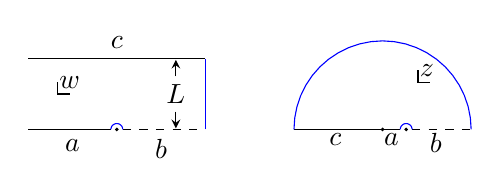
\begin{tikzpicture}[scale = 0.75]
\draw (0,0) -- (1.4,0);
\draw[dashed] (1.6,0) -- (3,0);
\draw[fill] (1.5,0) circle (0.02);
\draw[blue] [domain=0:180] plot ({1.5+0.1*cos(\x)}, {0.1*sin(\x)});
\draw (0,1.2) -- (3,1.2);
\draw[-stealth] (2.5,0.9)--(2.5, 1.18);
\draw[-stealth] (2.5,0.3)--(2.5, 0.02);
\node () at (2.5,0.6) {$L$};
\node[below] () at (0.75,0) {$a$};
\node[below] () at (2.25,0) {$b$};
\node[above] () at (1.5,1.2) {$c$};
\draw[blue] (3,0)--++(0,1.2);
\begin{scope}[shift={(0.5,0.6)}]
\node () at (0.2,0.2) {$w$};
\draw (0,0.2)--(0,0)--(0.2,0);
\end{scope}
\begin{scope}[shift={(6,0)}]
\draw (-1.5,0)--(0.3,0);
\draw[dashed] (0.5,0)--(1.5,0);
\draw[fill] (.4,0) circle (0.02);
\draw[fill] (0,0) circle (0.02);
\draw[blue] [domain=0:180] plot ({0.4+0.1*cos(\x)}, {0.1*sin(\x)});
\draw[blue] [domain=0:180] plot ({1.5*cos(\x)}, {1.5*sin(\x)});
\begin{scope}[shift={(0.6,0.8)}]
\node () at (0.15,0.2) {$z$};
\draw (0,0.2)--(0,0)--(0.2,0);
\node[below] () at (-0.45,-0.7) {$a$};
\node[below] () at (0.3,-0.7) {$b$};
\node[below] () at (-1.4,-0.7) {$c$};
\end{scope}
\end{scope}
\end{tikzpicture}


\end{document}